\citeauthor{siu2020virtual}, also motivated by the popularization of the VR technology, developed a White Cane to be used by BVI users in virtual environments and to make virtual reality application useful for these users as well. The traditional white cane transmits three sources of information to the user: Detection of obstacles, surface topography and foot-placement preview and these information are transmitted through sounds or haptics \cite{siu2020virtual} and the developed cane would simulate that in the virtual environment.

For the obstacle detection, the new cane was build with a three degree-of-freedom brake mechanism that would stop the movement when the cane hit an obstacle. It was installed a voice coil actuator that was used to detect surface properties or other information that had a higher frequency than the capacity of the brake mechanism. Lastly, a wave-based acoustic simulation was used to render geometry-aware sound effects in other to enable the user a sense the surroundings using the sounds (Echolocalisation).

The experiment's participants were meant to play a "Scavenger Hunt" using a HTC Vive. During the experiment each participant had two tasks:

\begin{itemize}
    \item Collect targets along the way;
    
    The main task. Five targets appeared, one at a time, once the previous target was collected, and they emitted a sound that acted as an audio beacon for the participant. The experiment was concluded when the participant collected all of them.
    
    \item Avoid virtual obstacles and walls.
    
    The secondary task. These obstacles didn't emit any sound as a beacon, but the participant could detect it by the shape and by the noise it emits when in contact with the cane. All the obstacles had the same geometry and material, a cube shaped metal. When tapped by the cane, this object emitted a metal clinking sound.
\end{itemize}

Besides the audio beacon and the metal sound, there were also a sound when a target was collected, when colliding with a wall and with an obstacle. Figure \ref{fig:siu_vr_targets} shows the targets obstacles and the starting point location.

The experiment was performed with 8 blind users (4 female, 4 male) from 25 to 70 years old. All of them did a training section where it was presented to them the mechanics of the virtual environment and how to detect walls, doors and obstacles. Figure \ref{fig:siu_vr_rooms} shows both the training and the game rooms.

\begin{figure}[h]
\centering
\begin{minipage}{.45\textwidth}
    \centering
    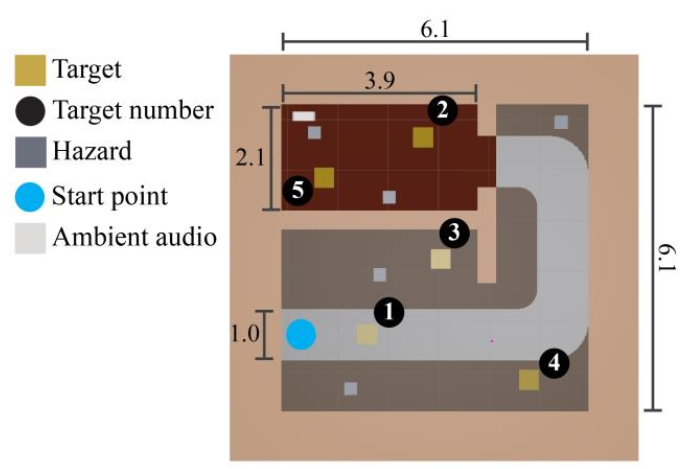
\includegraphics[width=\textwidth]{Revisao/VR Without Vision/VR without vision map.png}
    \captionof{figure}{Siu et al. key locations. Distances are in meters \cite{siu2020virtual}.}
    \label{fig:siu_vr_targets}
\end{minipage}
\hfil
\begin{minipage}{.45\textwidth}
    \centering
    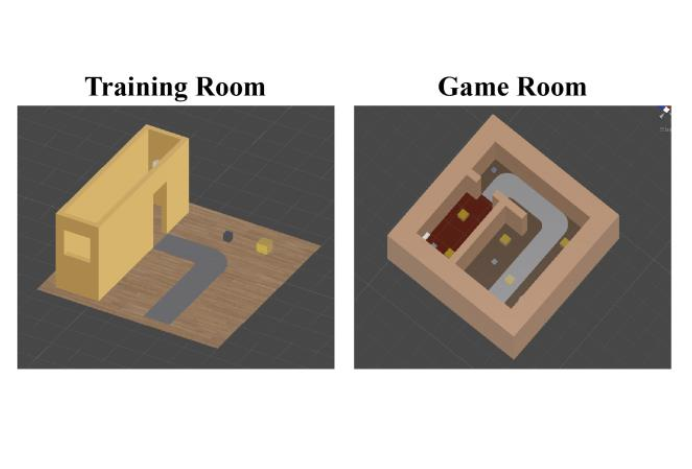
\includegraphics[width=\textwidth]{Revisao/VR Without Vision/VR without vision rooms.png}
    \captionof{figure}{Siu et al. training and game rooms layout \cite{siu2020virtual}.}
    \label{fig:siu_vr_rooms}
\end{minipage}
\end{figure}

The researcher found out that the simulated vibration of the cane confused part of the participants, while other part were familiar with that vibration of the cane. This was reflected in the performance of this participants. The ones that were already used with this vibration performed better. This shows that user preferences can impact their perfomance and experience in the VE. 

Another point taken by the researcher was about navigating in tight spaces. Is was easier for the participants to navigate in larger areas, similar as it is said in real world. 

The final conclusion was about the exploration of the environment. The participants were focused in finding all of the target and did not explore the environment. This might have caused a bias in the low time and low obstacle hits. So it not sure that the tool could help a BVI user to freely explore a VE.

The authors noted some limitation. The cane, even though it had a good brake system, it didn't stop the participant when he/she walked forwards towards a wall. The lack of variation in the cane material and in the feedback possibilities (i.e when the obstacle contact a point along the cane, not the tip of it).

The present experiment has similar motivations, to study or improve BVI users' navigation, but in different environments. While the work from \citeauthor{siu2020virtual} was focused in the navigation of BVI users inside a VE, this experiment uses VE to assess BVI navigation in a simulated real environment. \citeauthor{siu2020virtual} commented the importance of the sound in the guidance of the BVI and used spatialized audio to increase the realism and received a positive feedback by the participants as this experiment also did.

One big difference between the two works is the cane. \citeauthor{siu2020virtual} used a cane controller that represented a virtual cane inside the VE, as was made in this work with the \textit{Virtual Cane}, but the feedback from the \textit{Virtual Cane} interaction on the VE was only a vibration, whilst the cane controller, besides using a high frequency response that could be said to be similar to a vibration,  used a brake system to simulate the contact with the wall or obstacle. This experiment couldn't apply this resource for financial and time reasons.